
\chapter{Systemarkitektur}
\begin{longtabu} to \linewidth{@{}l l l X[l]@{}}
	
	
	Version &    Dato &    Ansvarlig &    Beskrivelse\\[-1ex]
	\midrule
	0.1 &    03-11-2015 &    MB &    Oprettelse \\[-1ex]
	0.2 &    10-11-2015 &    DHC, MB &    Start af skrivning, indsætning af billeder Hardware  \\[-1ex]
	0.3 &  11-11-2015   &  DHC   &   Forstrækning  \\[-1ex]
	
	\label{version_Systemark}
\end{longtabu}

\section{Hardware}
\subsection{Design}

Systemets hardware kan illustreres i et BBD. Det ses at nedestående figur at systemet består af fem hardware blokke: software system, forstærker, filter, DAQ og transducer. Disse fem blokke udgør til sammen selve blodtryksmåleren.  
	
\begin{figure}[htb]
	\centering
	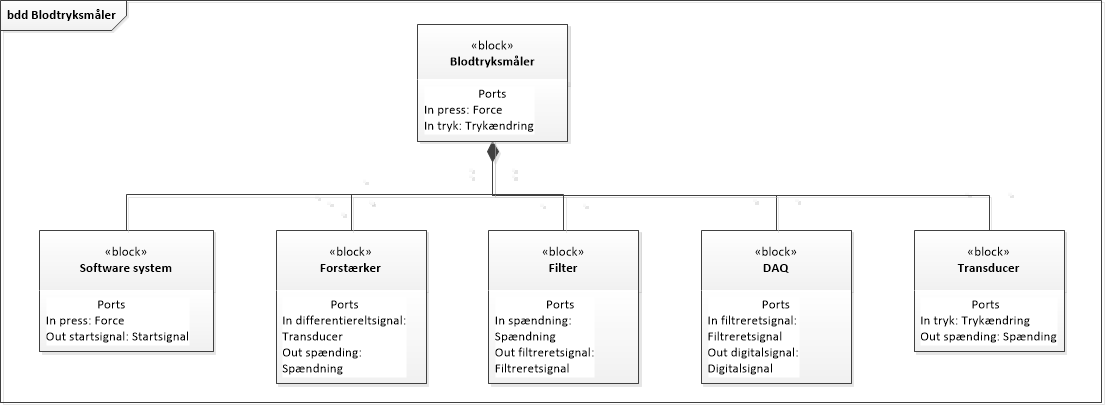
\includegraphics[width=1.0\textwidth]{Figurer/BDD}
	\caption{Block Definition Diagram for hardware}
	%\label{fig:BDD viser blodtrykssystemets hardwaredele, samt sammenhængen mellem disse}
\end{figure}

Ovenstående BDD-diagram fører videre til udarbejdelsen af IBD for hardware komponenterne. I dette diagram vises koblingen mellem de forskellige blokke gennem port forbindelser.  Det ses at signalet starter ved transduceren, hvorefter det bliver behandlet gennem forstærker, filter og DAQ. Til sidste sendes det ind i software systemet, som bliver påvirket at tryk på knapper på GUI. 

\begin{figure}[htb]
	\centering
	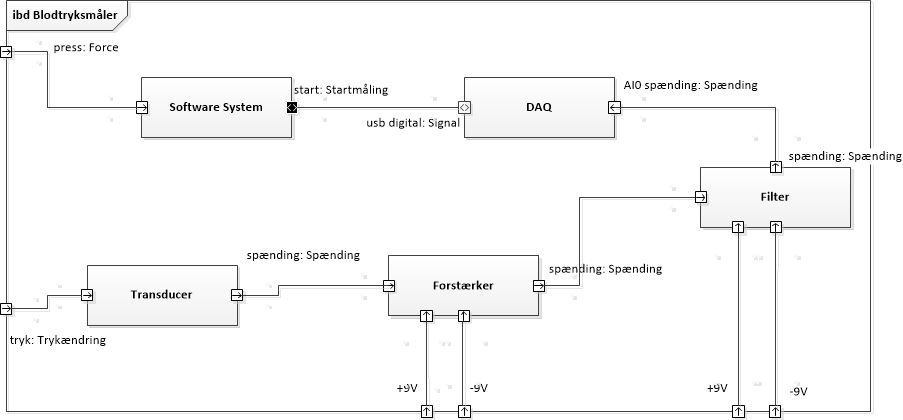
\includegraphics[width=1.0\textwidth]{Figurer/IBD}
	\caption{Infernal Block Diagram for hardware}
	\label{fig:IBD viser koblingen mellem blodtrykssystemets hardwaredele}
\end{figure}

\subsubsection{Forstærkning}
Transduceren måler en trykændring som den omsætter til en spænding. Dette er udtrykt ved et differentieret signal, som sendes ind i forstærkning-blokken. Da signalet fra transduceren ligger i et interval på 0 - 11.28 mV,  skal dette forstærkes op så det passer med NI-DAQ. I projektet er det valgt at DAQ'ens input skal ligge mellem 0-5V. Derved skal signalet forstærkes: 

\begin{equation}
11.28mV\cdot x = 5 V \Rightarrow x= 443
\end{equation}
Under simulering bruges Analog Discovery som en funktionsgenerator, der simulere det differentieret signal. Analog Discovery har dog en vis usikkerhed, når der arbejdes med små spændinger. Dette kan modarbejdes med en spændingsdeler, hvor der bygges et kredsløb som ligger før selve forstærkningen. Dette gør at Analog Discovery kan sende en højere spænding, som så gøre mindre igen ved spændingsdeler princippet.  

\subsubsection{Lavpas}
I projektet skal der laves et 2. ordens lavpasfilter. Dette filter skal være et Salen-Key Buttenworth-filter, med en knækfrekvens på 50 Hz. 

\subsection{Implementering}
\subsubsection{Forstærkning}
For at få den rette forstærkning har vi valgt at benytte operationsforstærkeren INA-114. Her kan transduceren sættes på med det differentieret signal. Under opbygning og modultestning vil det differentieret signal blive simuleret af Analog Discovery.
For at få den rette forstærkning ændres der på den "indre" modstand ($ R_g $) til INA114.
 
For at imøde usikkerheden ved Analog Discovery, laves et lille kredsløb efter spændingsdeler princippet. Her bruges $ R_1=10k\Omega $ og $ R_2 = 1k\Omega $. Da vi kender det signal som skal ind i INA-114 og modstanden kan vi derved finde størrelsen af den spænding som skal sende fra Analog Discovery.
 
\begin{equation}
U_{INA} = U_{analog} \cdot \frac{R_2}{R_1 + R_2} \Rightarrow 5mV = U_{analog}\cdot \frac{R_2}{R_1+R_2} \Rightarrow U_{analog}= 55mV
\end{equation} 

\subsubsection{Lavpas}
For at opnå den ønskede effekt i lavpasfilteret, blev det oplyst at $ f_c=50$ Hz, $ R_1 = R_2 $ og $ C_2=680 nF$. Ud fra det udregnes de resterende komponentværdier for filteret.  


\subsection{Modultest}
\subsubsection{Forstærkning}
\subsubsection{Lavpas}
For at teste lavpasfilteret foretages målinger med en sinus, hvor frekvensen variere for hver måling. Derved aflæses fasen, mellem indgang- og udgangssignal, og amplituden for hver måling. 
Ved knækfrekvensen skal fasendrejningen være 90\textdegree. Amplituden skal ændre sig XXX. Dette kan aflæses på billedet Måling for 50 Hz.
Efter knækfrekvensen skal amplituden blive mindre og mindre(går mod nul). På Måling for 60 Hz, kan det ses hvordan amplituden er faldet drastisk efter knækfrekvensen.  \\
\begin{figure}[htb]
	\centering
	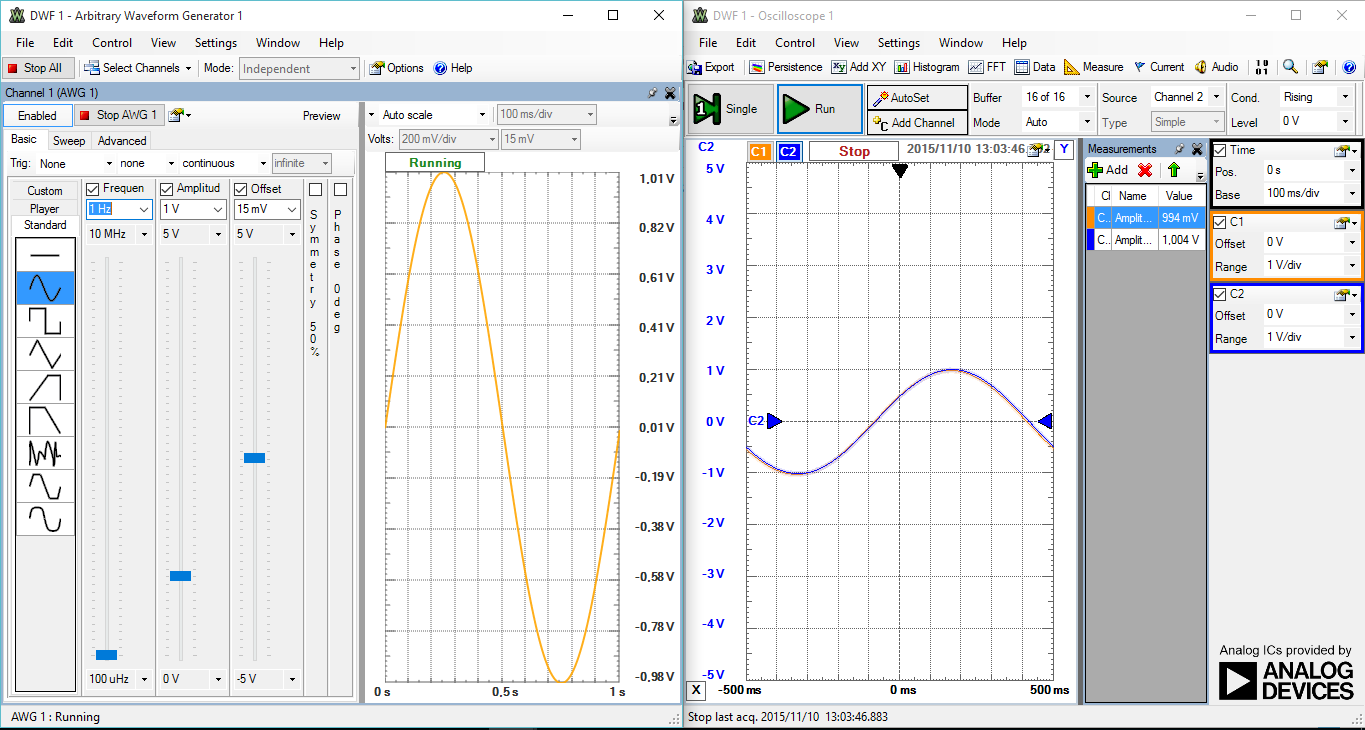
\includegraphics[width=1.0\textwidth]{Figurer/10Hz}
	\caption{Måling for 10 Hz}
	\label{fig:maeling10Hz}
\end{figure}

\begin{figure}[htb]
	\centering
	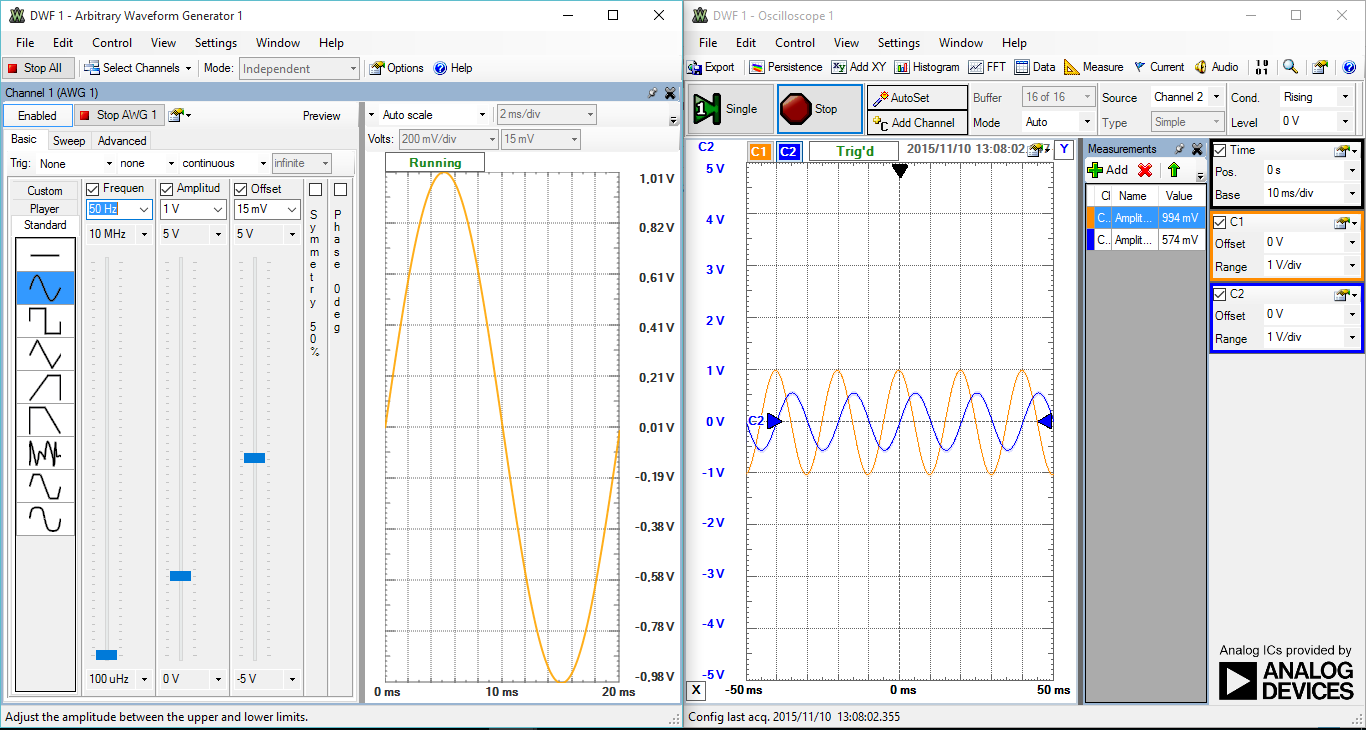
\includegraphics[width=1.0\textwidth]{Figurer/50Hz}
	\caption{Måling for 50 Hz}
	\label{fig:maeling50Hz}
\end{figure}

\begin{figure}[htb]
	\centering
	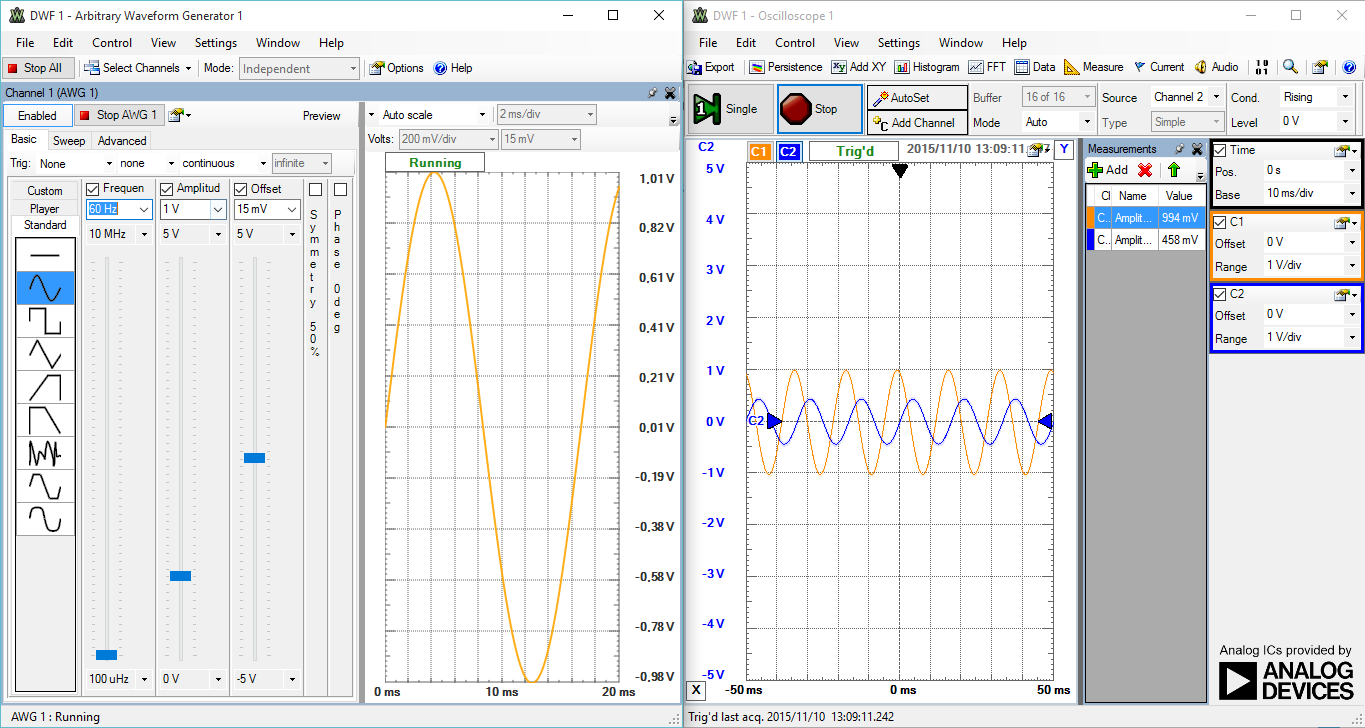
\includegraphics[width=1.0\textwidth]{Figurer/60Hz}
	\caption{Måling for 60 Hz}
	\label{fig:maeling60Hz}
\end{figure}
